%%%%%%%%%%%%%%%%%%%%%%%%%%%%%%%%%%%%%%%%%%%%%%%%%%%%%%%%%%%%%%%%%%%%%%%%%%%%%%%%%%%%%
% This creates an English IPA chart for vowels                                      %
%                                                                                   %
% Compiled from material_IPA_en_chart.tex when a                                    %
% standalone document is needed                                                     %
%                                                                                   %
% Code is only slightly from:                                                       %
%   https://tex.stackexchange.com/questions/156955/tikz-pgf-linguistics-vowel-chart %
%                                                                                   %
% -Joshua McNeill (joshua dot mcneill at uga dot edu)                               %
%%%%%%%%%%%%%%%%%%%%%%%%%%%%%%%%%%%%%%%%%%%%%%%%%%%%%%%%%%%%%%%%%%%%%%%%%%%%%%%%%%%%%

% Custom command
\def\V(#1,#2){barycentric cs:hf={(3-#1)*(2-#2)},hb={(3-#1)*#2},lf={#1*(2-#2)},lb={#1*#2}}

% Chart
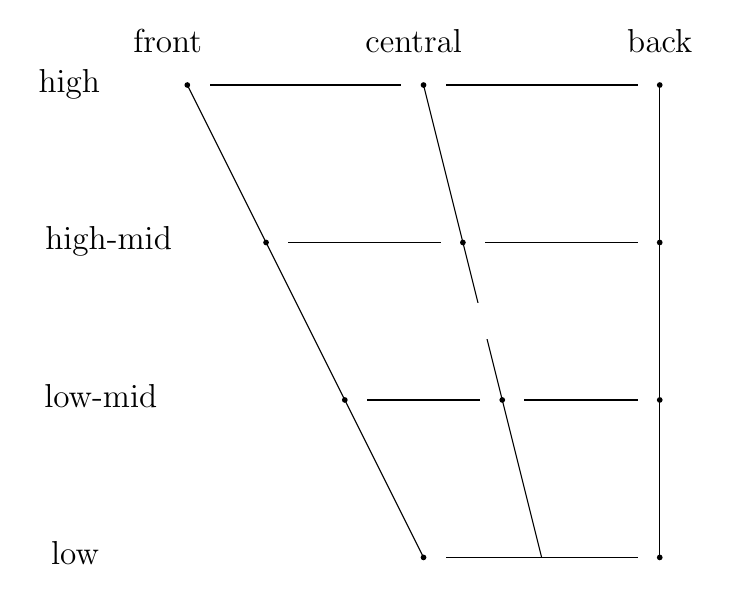
\begin{tikzpicture}[scale=3]
  \large
  \tikzset{
    vowel/.style={fill=white, anchor=mid, text depth=0ex, text height=1ex},
    dot/.style={circle,fill=black,minimum size=0.4ex,inner sep=0pt,outer sep=-1pt},
  }
  \coordinate (hf) at (0,2); % high front
  \coordinate (hb) at (2,2); % high back
  \coordinate (lf) at (1,0); % low front
  \coordinate (lb) at (2,0); % low back
  \def\V(#1,#2){barycentric cs:hf={(3-#1)*(2-#2)},hb={(3-#1)*#2},lf={#1*(2-#2)},lb={#1*#2}}

  % Draw the horizontal lines first.
  \draw (\V(0,0)) -- (\V(0,2));
  \draw (\V(1,0)) -- (\V(1,2));
  \draw (\V(2,0)) -- (\V(2,2));
  \draw (\V(3,0)) -- (\V(3,2));

  % Place all the unrounded-rounded pairs next, on top of the horizontal lines.
  \path (\V(0,0))     node[vowel, left] { } node[vowel, right] { } node[dot] {};
  \path (\V(0,1))     node[vowel, left] { } node[vowel, right] { } node[dot] {};
  \path (\V(0,2))     node[vowel, left] { } node[vowel, right] { } node[dot] {};
  \path (\V(0.5,0.4)) node[vowel, left] { } node[vowel, right] { } node[   ] {};
  \path (\V(0.5,1.6)) node[vowel, left] { } node[vowel, right] { } node[   ] {};
  \path (\V(1,0))     node[vowel, left] { } node[vowel, right] { } node[dot] {};
  \path (\V(1,1))     node[vowel, left] { } node[vowel, right] { } node[dot] {};
  \path (\V(1,2))     node[vowel, left] { } node[vowel, right] { } node[dot] {};
  \path (\V(2,0))     node[vowel, left] { } node[vowel, right] { } node[dot] {};
  \path (\V(2,1))     node[vowel, left] { } node[vowel, right] { } node[dot] {};
  \path (\V(2,2))     node[vowel, left] { } node[vowel, right] { } node[dot] {};
  \path (\V(2.5,0))   node[vowel, left] { } node[vowel, right] { } node[   ] {};
  \path (\V(3,0))     node[vowel, left] { } node[vowel, right] { } node[dot] {};
  \path (\V(3,2))     node[vowel, left] { } node[vowel, right] { } node[dot] {};

  % Draw the vertical lines.
  \draw (\V(0,0)) -- (\V(3,0));
  \draw (\V(0,1)) -- (\V(3,1));
  \draw (\V(0,2)) -- (\V(3,2));

  % Place the unpaired symbols last, on top of the vertical lines.
  \path (\V(1.5,1))   node[vowel]       { };
  \path (\V(-0.25,0)) node[vowel]       {front};
  \path (\V(-0.25,1)) node[vowel]       {central};
  \path (\V(-0.25,2)) node[vowel]       {back};
  \path (\V(0,-0.5))  node[vowel]       {high};
  \path (\V(1,-0.8))  node[vowel]       {high-mid};
  \path (\V(2,-1.55)) node[vowel]       {low-mid};
  \path (\V(3,-2.95)) node[vowel]       {low};
\end{tikzpicture}
